\documentclass[11pt]{article}
\usepackage[textwidth=18.0cm, textheight=23.0cm, top=2.0cm]{geometry}
\usepackage{pst-all}
\usepackage{amssymb}
\usepackage{tikz}
\usepackage{underscore}\begin{document}
\pagestyle{empty}


ClassName: \underline{\textbf{Class_10.2bp-37}}
\par
BinSize: \underline{\textbf{100 × 100}}
\par
ReduceSize: \underline{\textbf{100 × 100}}
\par
TypeNum: \underline{\textbf{80}}
\par
Num: \underline{\textbf{80}}
\par
OutS: \underline{\textbf{100000}}
\par
InS: \underline{\textbf{93747}}
\par
Rate: \underline{\textbf{0.937}}
\par
UB: \underline{\textbf{10}}
\par
LB0: \underline{\textbf{10}}
\par
LB: \underline{\textbf{10}}
\par
LBWithCut: \underline{\textbf{10}}
\par
NodeCut: \underline{\textbf{0}}
\par
ExtendedNodeCnt: \underline{\textbf{1}}
\par
GenNodeCnt: \underline{\textbf{1}}
\par
PrimalNode: \underline{\textbf{0}}
\par
ColumnCount: \underline{\textbf{10}}
\par
TotalCutCount: \underline{\textbf{0}}
\par
RootCutCount: \underline{\textbf{0}}
\par
LPSolverCnt: \underline{\textbf{1}}
\par
PricingSolverCnt: \underline{\textbf{0}}
\par
BranchAndBoundNum: \underline{\textbf{1}}
\par
isOpt: \underline{\textbf{true}}
\par
TimeOnPrimal: \underline{\textbf{0.000 s}}
\par
TimeOnPricing: \underline{\textbf{0.000 s}}
\par
TimeOnRmp: \underline{\textbf{0.063 s}}
\par
TotalTime: \underline{\textbf{0.125 s}}
\par
\newpage


\begin{tikzpicture}[shorten >=1pt,scale=1.0,every node/.style={scale=1.0},->]
\tikzstyle{vertex}=[circle,fill=black!25,minimum size=14pt,inner sep=0pt]
\filldraw[fill=gray!40!white, draw=black] (0,0) rectangle (15.0,15.0);
\foreach \name/\x/\y/\w/\h in {98x100/0.0/0.0/14.7/15.0,2x40/14.7/0.0/0.3/6.0}
\filldraw[fill=white!40!white, draw=black] (\x,\y) rectangle node[draw] (\name) {\name} ++(\w,\h);
\end{tikzpicture}


w =98 , h =100 , x =0 , y =0 , v =9800
\par
w =2 , h =40 , x =98 , y =0 , v =80
\par
\newpage


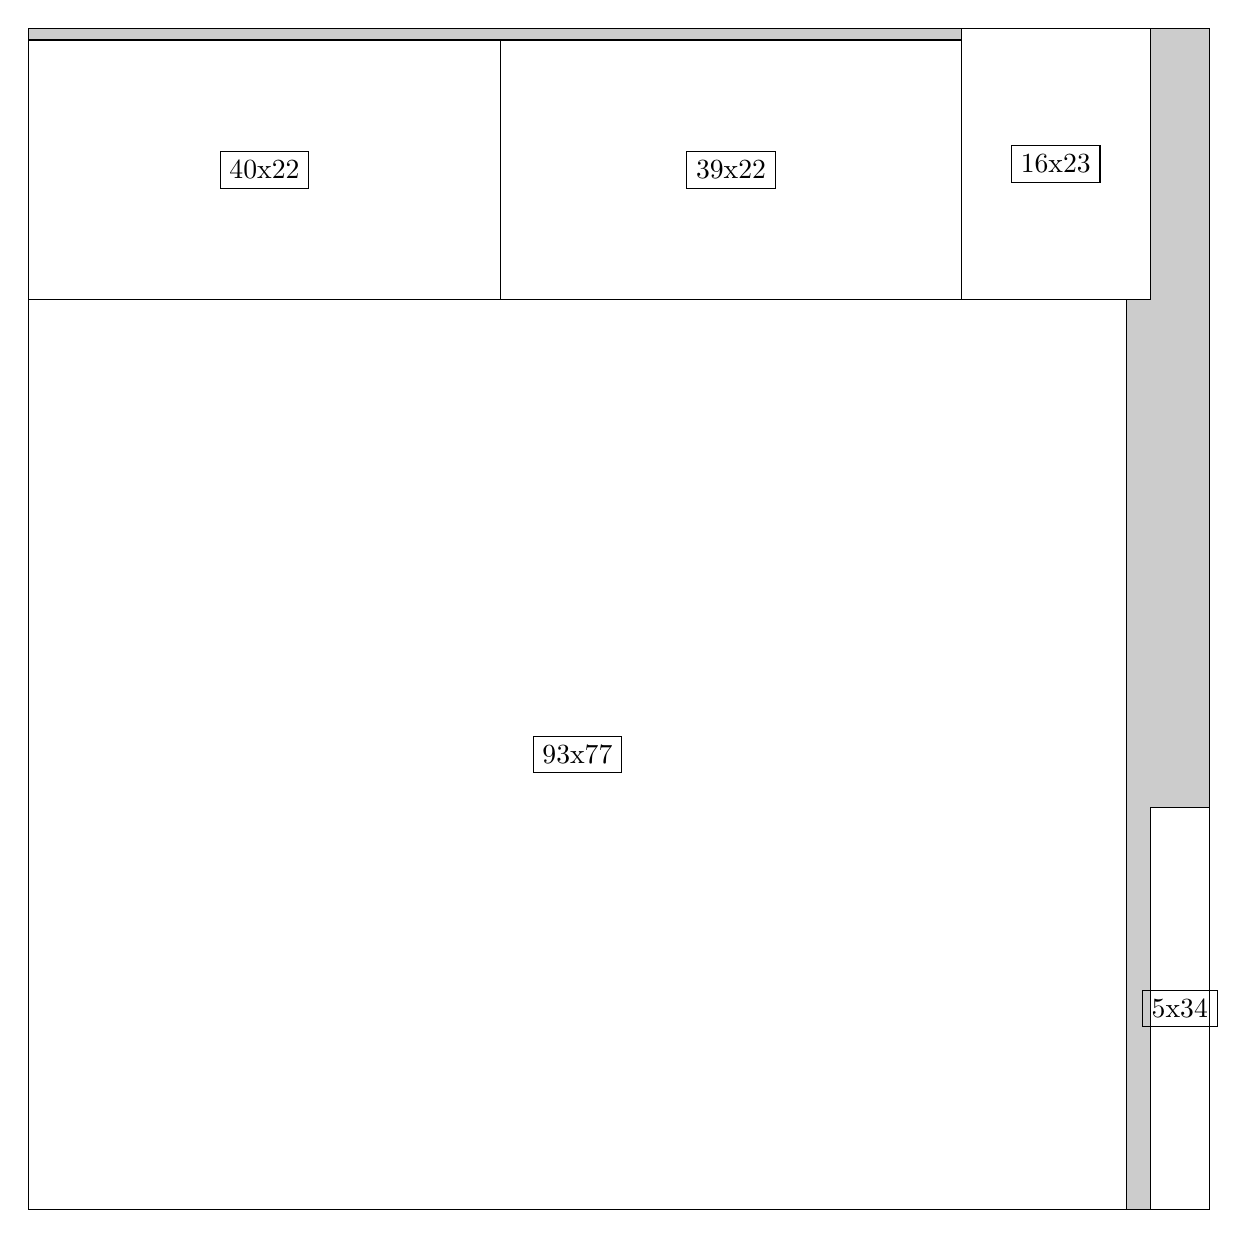
\begin{tikzpicture}[shorten >=1pt,scale=1.0,every node/.style={scale=1.0},->]
\tikzstyle{vertex}=[circle,fill=black!25,minimum size=14pt,inner sep=0pt]
\filldraw[fill=gray!40!white, draw=black] (0,0) rectangle (15.0,15.0);
\foreach \name/\x/\y/\w/\h in {93x77/0.0/0.0/13.95/11.549999999999999,40x22/0.0/11.549999999999999/6.0/3.3,39x22/6.0/11.549999999999999/5.85/3.3,16x23/11.85/11.549999999999999/2.4/3.4499999999999997,5x34/14.25/0.0/0.75/5.1}
\filldraw[fill=white!40!white, draw=black] (\x,\y) rectangle node[draw] (\name) {\name} ++(\w,\h);
\end{tikzpicture}


w =93 , h =77 , x =0 , y =0 , v =7161
\par
w =40 , h =22 , x =0 , y =77 , v =880
\par
w =39 , h =22 , x =40 , y =77 , v =858
\par
w =16 , h =23 , x =79 , y =77 , v =368
\par
w =5 , h =34 , x =95 , y =0 , v =170
\par
\newpage


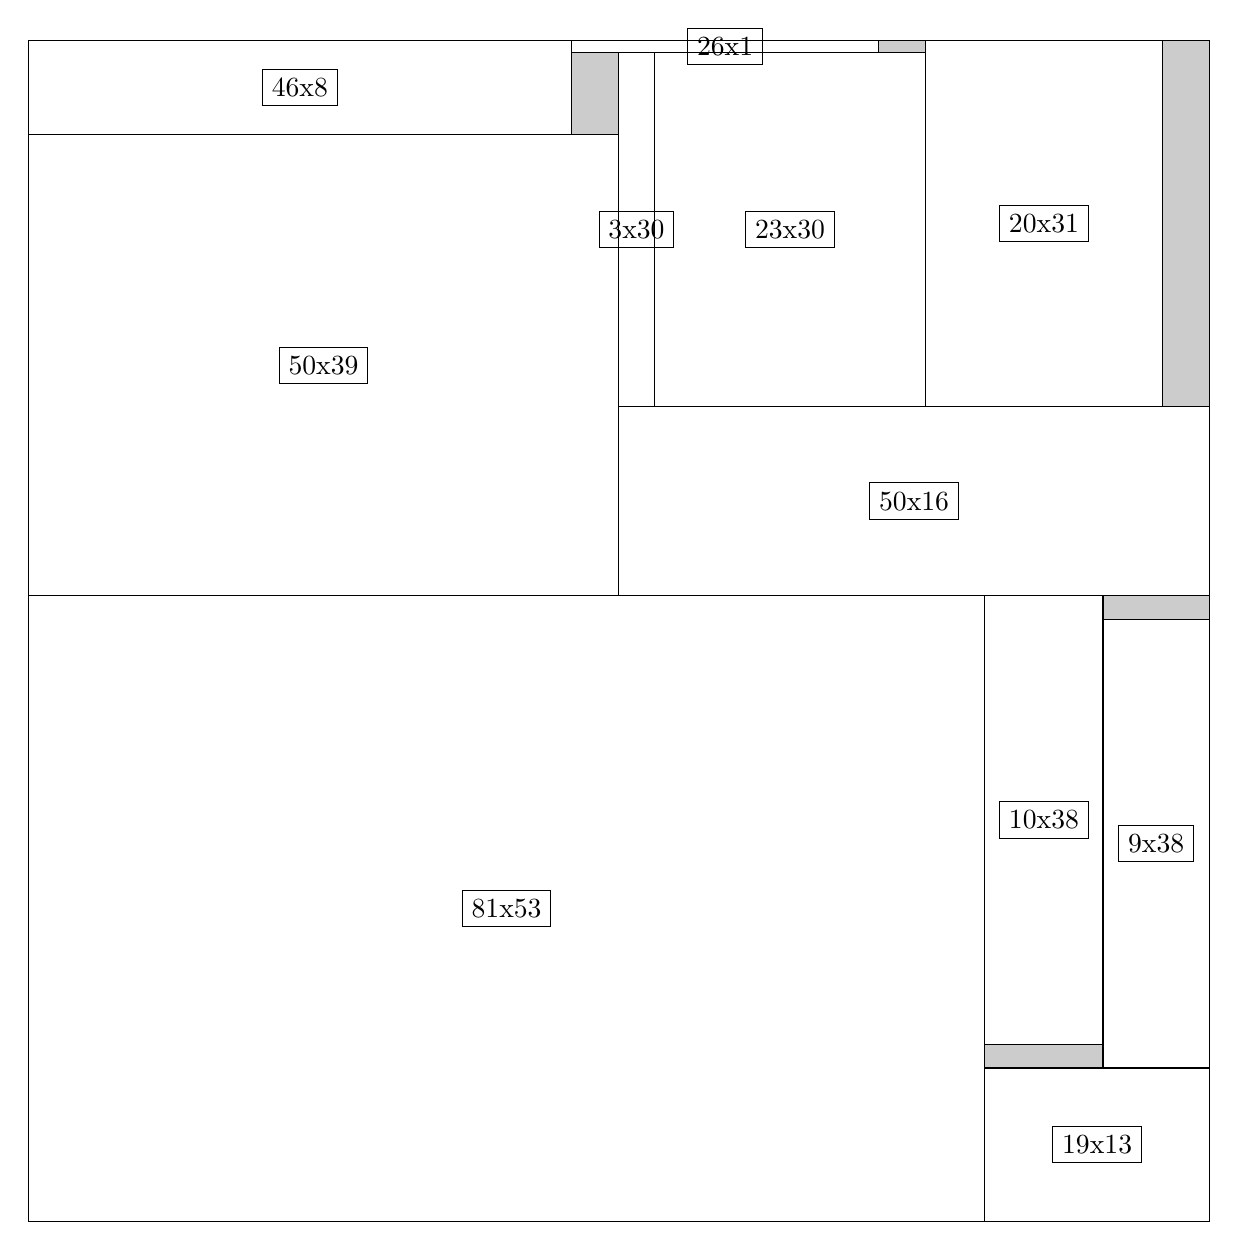
\begin{tikzpicture}[shorten >=1pt,scale=1.0,every node/.style={scale=1.0},->]
\tikzstyle{vertex}=[circle,fill=black!25,minimum size=14pt,inner sep=0pt]
\filldraw[fill=gray!40!white, draw=black] (0,0) rectangle (15.0,15.0);
\foreach \name/\x/\y/\w/\h in {81x53/0.0/0.0/12.15/7.949999999999999,50x39/0.0/7.949999999999999/7.5/5.85,20x31/11.4/10.35/3.0/4.6499999999999995,50x16/7.5/7.949999999999999/7.5/2.4,23x30/7.949999999999999/10.35/3.4499999999999997/4.5,10x38/12.15/2.25/1.5/5.7,46x8/0.0/13.799999999999999/6.8999999999999995/1.2,9x38/13.65/1.95/1.3499999999999999/5.7,19x13/12.15/0.0/2.85/1.95,3x30/7.5/10.35/0.44999999999999996/4.5,26x1/6.8999999999999995/14.85/3.9/0.15}
\filldraw[fill=white!40!white, draw=black] (\x,\y) rectangle node[draw] (\name) {\name} ++(\w,\h);
\end{tikzpicture}


w =81 , h =53 , x =0 , y =0 , v =4293
\par
w =50 , h =39 , x =0 , y =53 , v =1950
\par
w =20 , h =31 , x =76 , y =69 , v =620
\par
w =50 , h =16 , x =50 , y =53 , v =800
\par
w =23 , h =30 , x =53 , y =69 , v =690
\par
w =10 , h =38 , x =81 , y =15 , v =380
\par
w =46 , h =8 , x =0 , y =92 , v =368
\par
w =9 , h =38 , x =91 , y =13 , v =342
\par
w =19 , h =13 , x =81 , y =0 , v =247
\par
w =3 , h =30 , x =50 , y =69 , v =90
\par
w =26 , h =1 , x =46 , y =99 , v =26
\par
\newpage


\begin{tikzpicture}[shorten >=1pt,scale=1.0,every node/.style={scale=1.0},->]
\tikzstyle{vertex}=[circle,fill=black!25,minimum size=14pt,inner sep=0pt]
\filldraw[fill=gray!40!white, draw=black] (0,0) rectangle (15.0,15.0);
\foreach \name/\x/\y/\w/\h in {50x100/7.5/0.0/7.5/15.0,50x75/0.0/0.0/7.5/11.25,37x25/1.95/11.25/5.55/3.75,12x18/0.0/11.25/1.7999999999999998/2.6999999999999997,11x3/0.0/13.95/1.65/0.44999999999999996}
\filldraw[fill=white!40!white, draw=black] (\x,\y) rectangle node[draw] (\name) {\name} ++(\w,\h);
\end{tikzpicture}


w =50 , h =100 , x =50 , y =0 , v =5000
\par
w =50 , h =75 , x =0 , y =0 , v =3750
\par
w =37 , h =25 , x =13 , y =75 , v =925
\par
w =12 , h =18 , x =0 , y =75 , v =216
\par
w =11 , h =3 , x =0 , y =93 , v =33
\par
\newpage


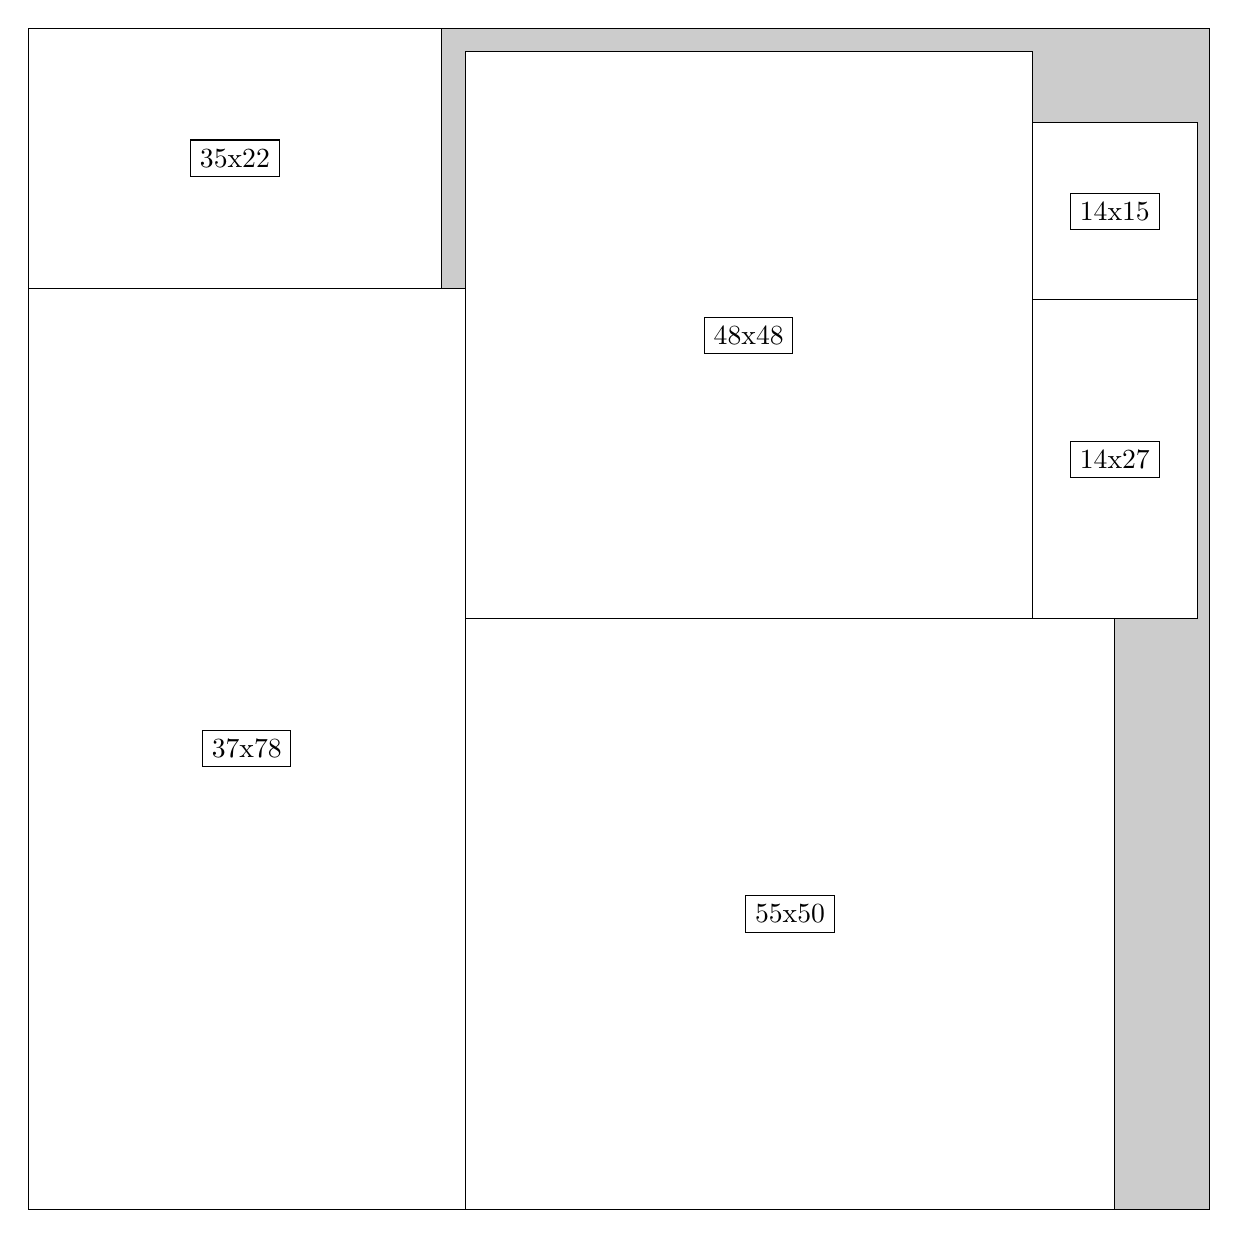
\begin{tikzpicture}[shorten >=1pt,scale=1.0,every node/.style={scale=1.0},->]
\tikzstyle{vertex}=[circle,fill=black!25,minimum size=14pt,inner sep=0pt]
\filldraw[fill=gray!40!white, draw=black] (0,0) rectangle (15.0,15.0);
\foreach \name/\x/\y/\w/\h in {37x78/0.0/0.0/5.55/11.7,55x50/5.55/0.0/8.25/7.5,48x48/5.55/7.5/7.199999999999999/7.199999999999999,35x22/0.0/11.7/5.25/3.3,14x27/12.75/7.5/2.1/4.05,14x15/12.75/11.549999999999999/2.1/2.25}
\filldraw[fill=white!40!white, draw=black] (\x,\y) rectangle node[draw] (\name) {\name} ++(\w,\h);
\end{tikzpicture}


w =37 , h =78 , x =0 , y =0 , v =2886
\par
w =55 , h =50 , x =37 , y =0 , v =2750
\par
w =48 , h =48 , x =37 , y =50 , v =2304
\par
w =35 , h =22 , x =0 , y =78 , v =770
\par
w =14 , h =27 , x =85 , y =50 , v =378
\par
w =14 , h =15 , x =85 , y =77 , v =210
\par
\newpage


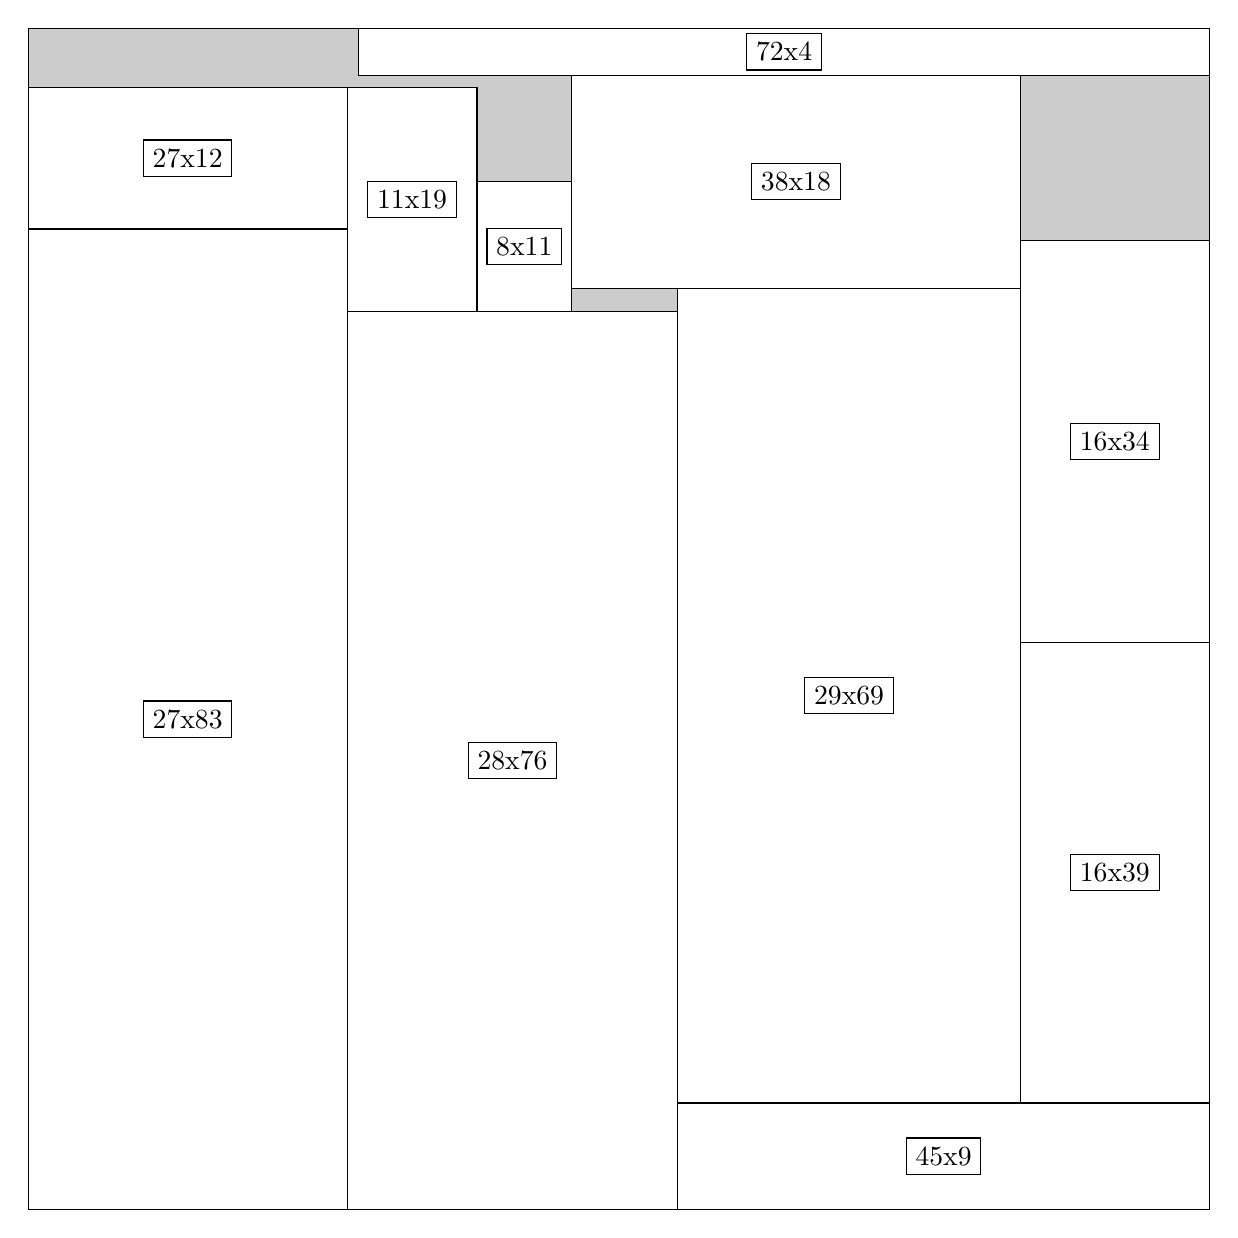
\begin{tikzpicture}[shorten >=1pt,scale=1.0,every node/.style={scale=1.0},->]
\tikzstyle{vertex}=[circle,fill=black!25,minimum size=14pt,inner sep=0pt]
\filldraw[fill=gray!40!white, draw=black] (0,0) rectangle (15.0,15.0);
\foreach \name/\x/\y/\w/\h in {27x83/0.0/0.0/4.05/12.45,28x76/4.05/0.0/4.2/11.4,29x69/8.25/1.3499999999999999/4.35/10.35,38x18/6.8999999999999995/11.7/5.7/2.6999999999999997,16x39/12.6/1.3499999999999999/2.4/5.85,16x34/12.6/7.199999999999999/2.4/5.1,45x9/8.25/0.0/6.75/1.3499999999999999,27x12/0.0/12.45/4.05/1.7999999999999998,72x4/4.2/14.399999999999999/10.799999999999999/0.6,11x19/4.05/11.4/1.65/2.85,8x11/5.7/11.4/1.2/1.65}
\filldraw[fill=white!40!white, draw=black] (\x,\y) rectangle node[draw] (\name) {\name} ++(\w,\h);
\end{tikzpicture}


w =27 , h =83 , x =0 , y =0 , v =2241
\par
w =28 , h =76 , x =27 , y =0 , v =2128
\par
w =29 , h =69 , x =55 , y =9 , v =2001
\par
w =38 , h =18 , x =46 , y =78 , v =684
\par
w =16 , h =39 , x =84 , y =9 , v =624
\par
w =16 , h =34 , x =84 , y =48 , v =544
\par
w =45 , h =9 , x =55 , y =0 , v =405
\par
w =27 , h =12 , x =0 , y =83 , v =324
\par
w =72 , h =4 , x =28 , y =96 , v =288
\par
w =11 , h =19 , x =27 , y =76 , v =209
\par
w =8 , h =11 , x =38 , y =76 , v =88
\par
\newpage


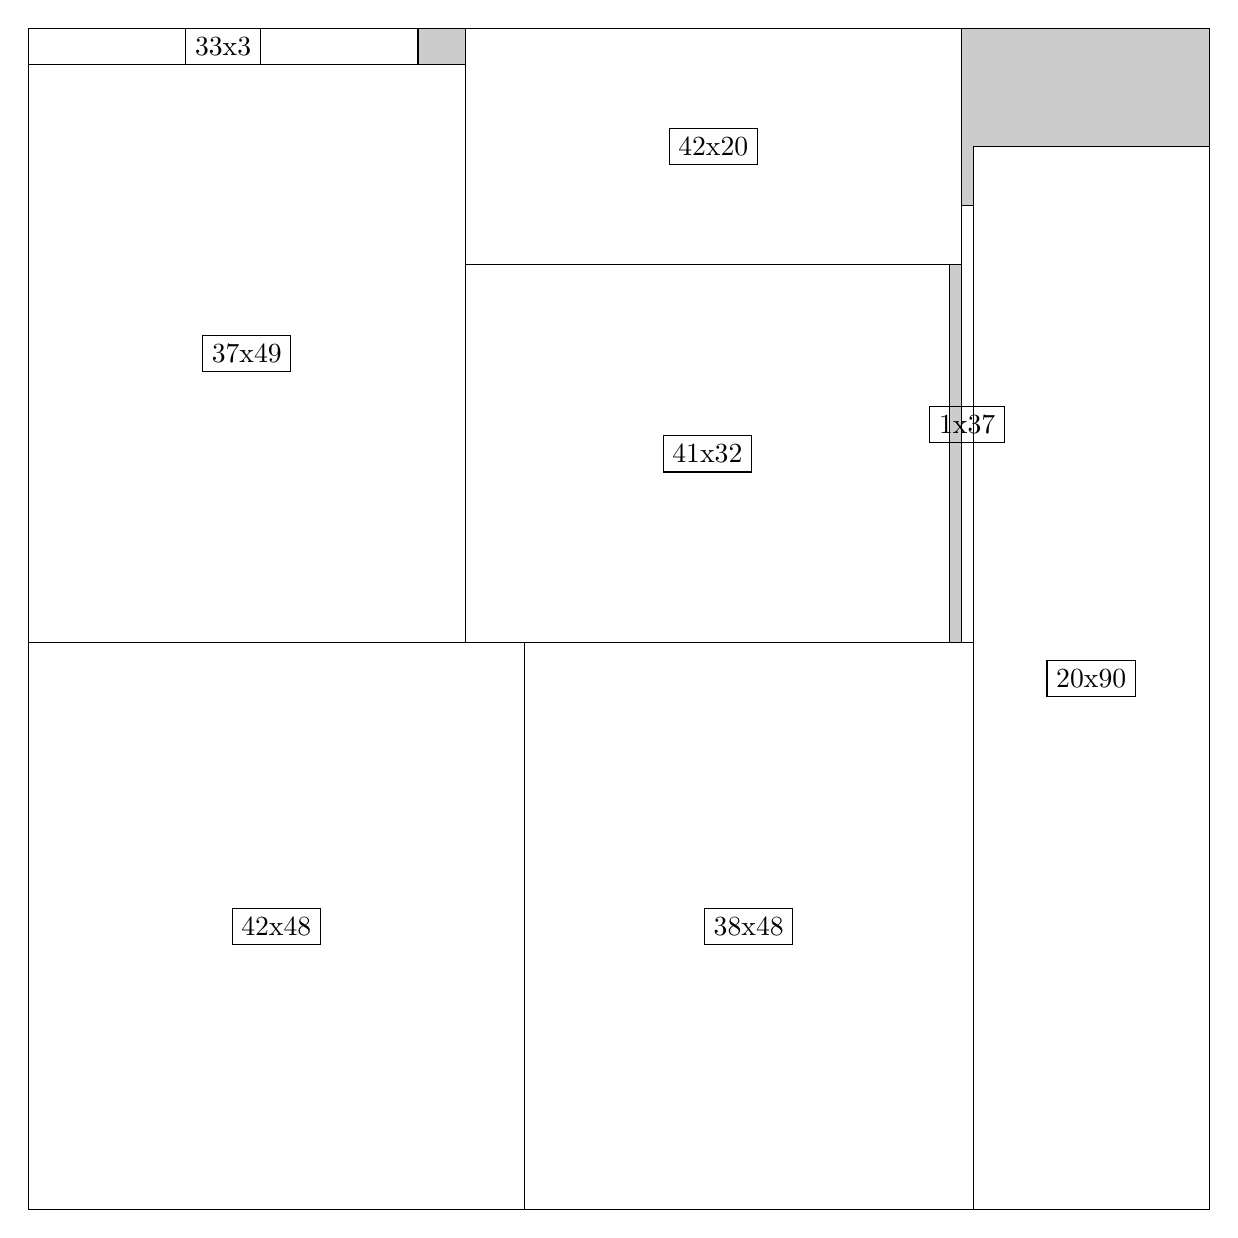
\begin{tikzpicture}[shorten >=1pt,scale=1.0,every node/.style={scale=1.0},->]
\tikzstyle{vertex}=[circle,fill=black!25,minimum size=14pt,inner sep=0pt]
\filldraw[fill=gray!40!white, draw=black] (0,0) rectangle (15.0,15.0);
\foreach \name/\x/\y/\w/\h in {42x48/0.0/0.0/6.3/7.199999999999999,38x48/6.3/0.0/5.7/7.199999999999999,37x49/0.0/7.199999999999999/5.55/7.35,20x90/12.0/0.0/3.0/13.5,41x32/5.55/7.199999999999999/6.1499999999999995/4.8,42x20/5.55/12.0/6.3/3.0,33x3/0.0/14.549999999999999/4.95/0.44999999999999996,1x37/11.85/7.199999999999999/0.15/5.55}
\filldraw[fill=white!40!white, draw=black] (\x,\y) rectangle node[draw] (\name) {\name} ++(\w,\h);
\end{tikzpicture}


w =42 , h =48 , x =0 , y =0 , v =2016
\par
w =38 , h =48 , x =42 , y =0 , v =1824
\par
w =37 , h =49 , x =0 , y =48 , v =1813
\par
w =20 , h =90 , x =80 , y =0 , v =1800
\par
w =41 , h =32 , x =37 , y =48 , v =1312
\par
w =42 , h =20 , x =37 , y =80 , v =840
\par
w =33 , h =3 , x =0 , y =97 , v =99
\par
w =1 , h =37 , x =79 , y =48 , v =37
\par
\newpage


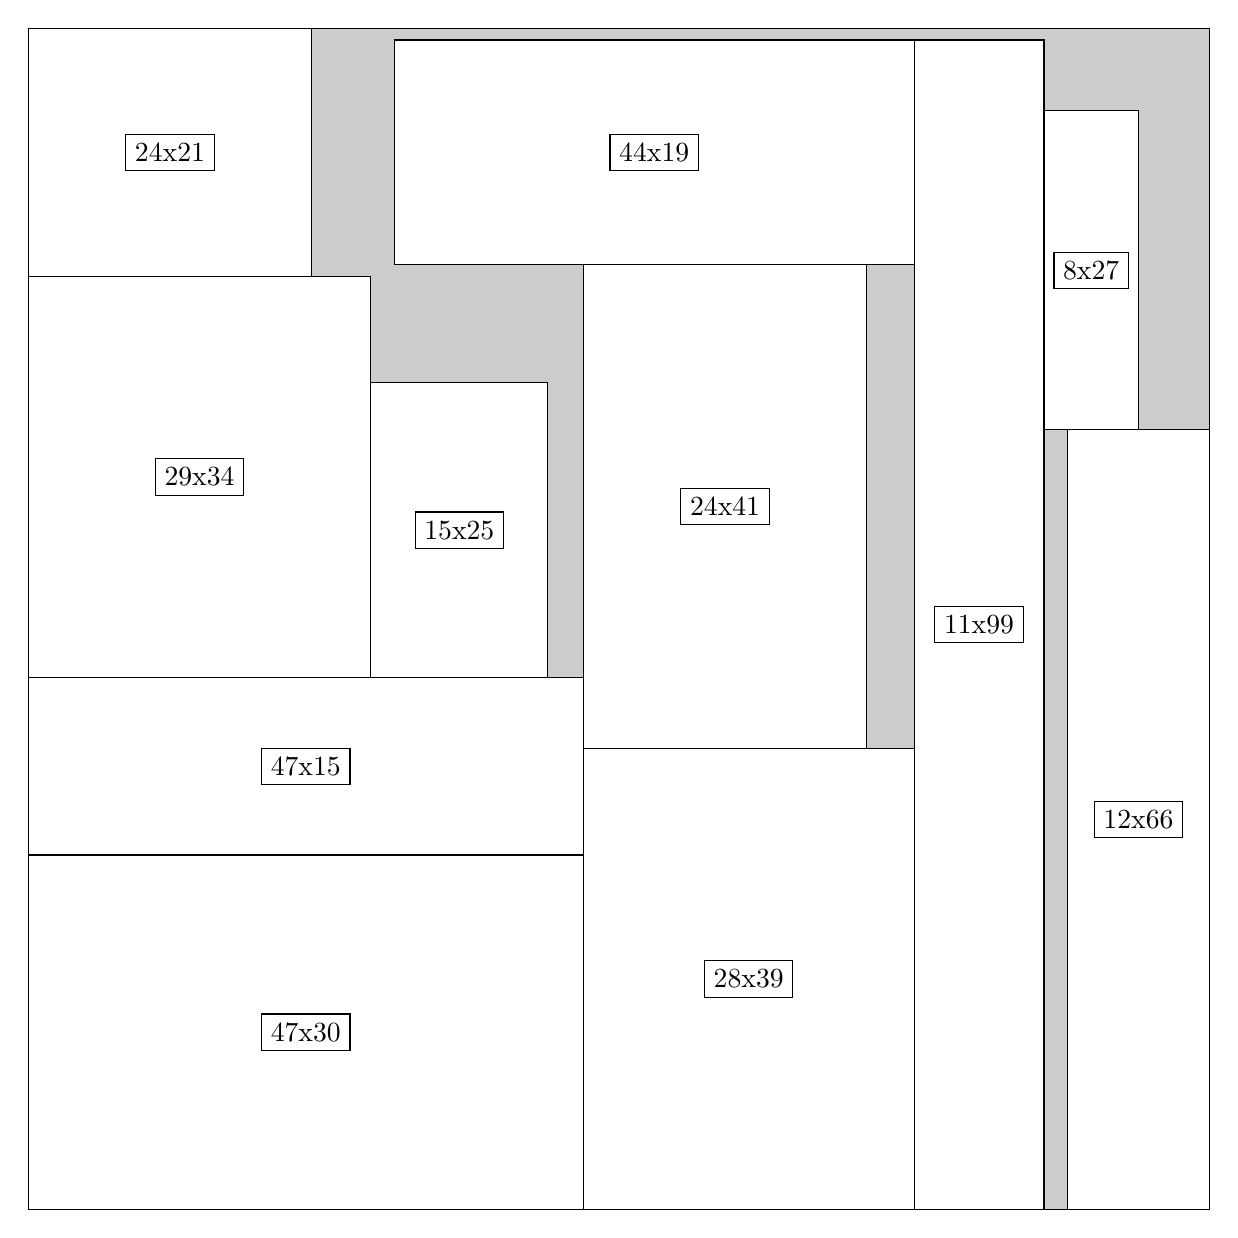
\begin{tikzpicture}[shorten >=1pt,scale=1.0,every node/.style={scale=1.0},->]
\tikzstyle{vertex}=[circle,fill=black!25,minimum size=14pt,inner sep=0pt]
\filldraw[fill=gray!40!white, draw=black] (0,0) rectangle (15.0,15.0);
\foreach \name/\x/\y/\w/\h in {47x30/0.0/0.0/7.05/4.5,28x39/7.05/0.0/4.2/5.85,11x99/11.25/0.0/1.65/14.85,29x34/0.0/6.75/4.35/5.1,24x41/7.05/5.85/3.5999999999999996/6.1499999999999995,44x19/4.6499999999999995/12.0/6.6/2.85,12x66/13.2/0.0/1.7999999999999998/9.9,47x15/0.0/4.5/7.05/2.25,24x21/0.0/11.85/3.5999999999999996/3.15,15x25/4.35/6.75/2.25/3.75,8x27/12.9/9.9/1.2/4.05}
\filldraw[fill=white!40!white, draw=black] (\x,\y) rectangle node[draw] (\name) {\name} ++(\w,\h);
\end{tikzpicture}


w =47 , h =30 , x =0 , y =0 , v =1410
\par
w =28 , h =39 , x =47 , y =0 , v =1092
\par
w =11 , h =99 , x =75 , y =0 , v =1089
\par
w =29 , h =34 , x =0 , y =45 , v =986
\par
w =24 , h =41 , x =47 , y =39 , v =984
\par
w =44 , h =19 , x =31 , y =80 , v =836
\par
w =12 , h =66 , x =88 , y =0 , v =792
\par
w =47 , h =15 , x =0 , y =30 , v =705
\par
w =24 , h =21 , x =0 , y =79 , v =504
\par
w =15 , h =25 , x =29 , y =45 , v =375
\par
w =8 , h =27 , x =86 , y =66 , v =216
\par
\newpage


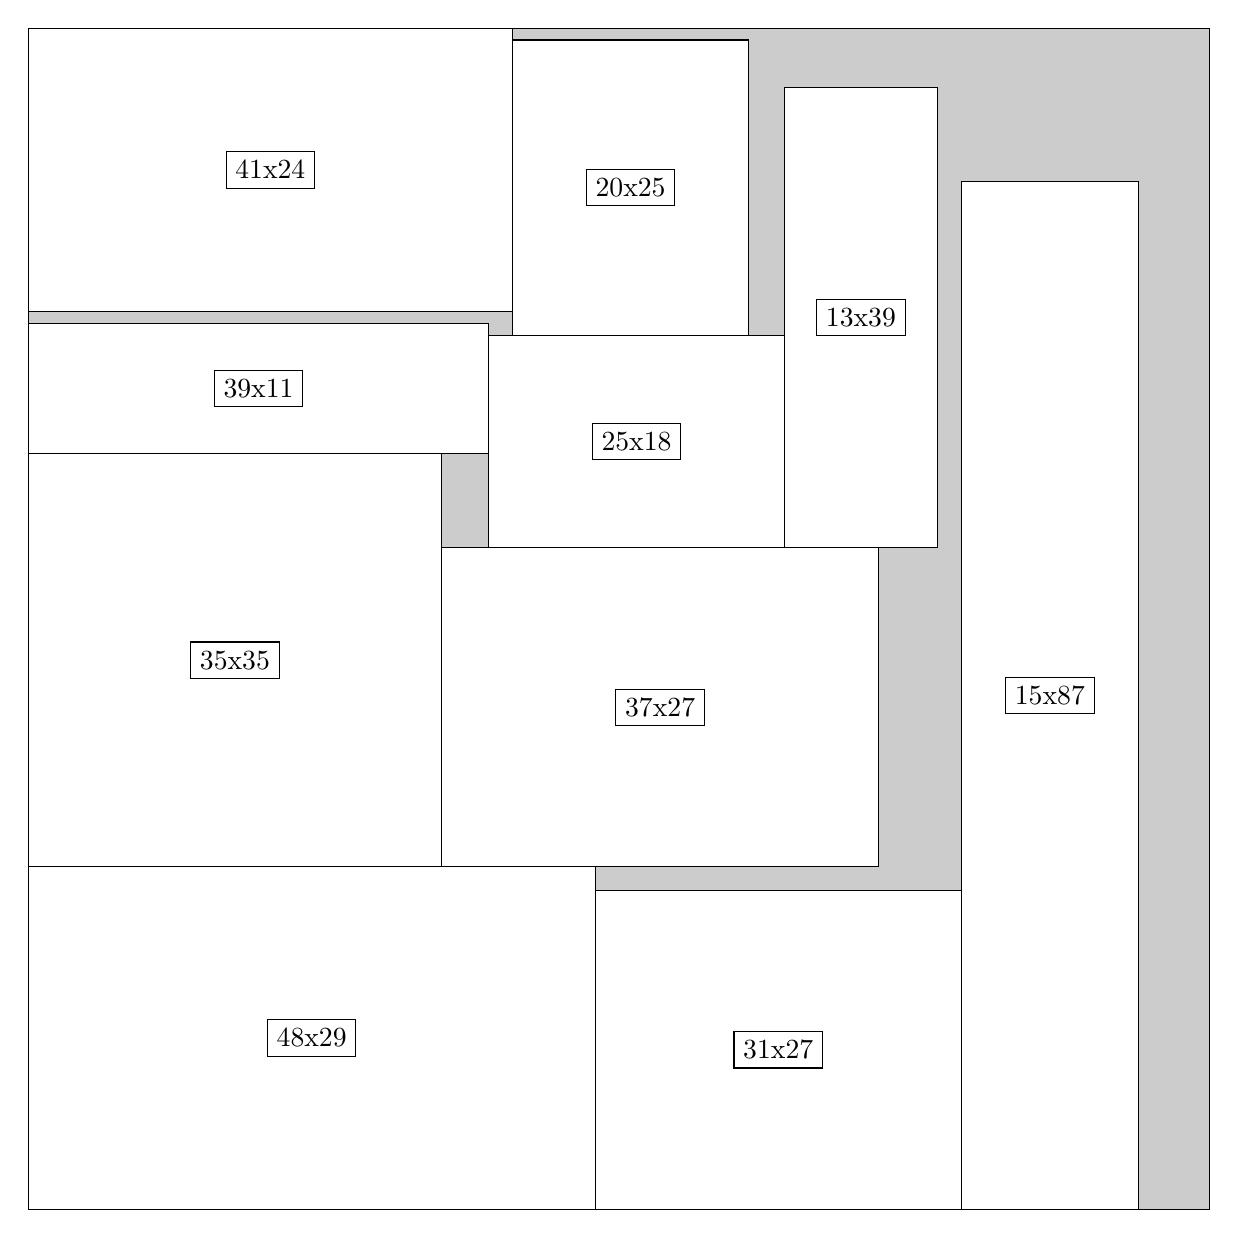
\begin{tikzpicture}[shorten >=1pt,scale=1.0,every node/.style={scale=1.0},->]
\tikzstyle{vertex}=[circle,fill=black!25,minimum size=14pt,inner sep=0pt]
\filldraw[fill=gray!40!white, draw=black] (0,0) rectangle (15.0,15.0);
\foreach \name/\x/\y/\w/\h in {48x29/0.0/0.0/7.199999999999999/4.35,15x87/11.85/0.0/2.25/13.049999999999999,35x35/0.0/4.35/5.25/5.25,37x27/5.25/4.35/5.55/4.05,41x24/0.0/11.4/6.1499999999999995/3.5999999999999996,31x27/7.199999999999999/0.0/4.6499999999999995/4.05,13x39/9.6/8.4/1.95/5.85,20x25/6.1499999999999995/11.1/3.0/3.75,25x18/5.85/8.4/3.75/2.6999999999999997,39x11/0.0/9.6/5.85/1.65}
\filldraw[fill=white!40!white, draw=black] (\x,\y) rectangle node[draw] (\name) {\name} ++(\w,\h);
\end{tikzpicture}


w =48 , h =29 , x =0 , y =0 , v =1392
\par
w =15 , h =87 , x =79 , y =0 , v =1305
\par
w =35 , h =35 , x =0 , y =29 , v =1225
\par
w =37 , h =27 , x =35 , y =29 , v =999
\par
w =41 , h =24 , x =0 , y =76 , v =984
\par
w =31 , h =27 , x =48 , y =0 , v =837
\par
w =13 , h =39 , x =64 , y =56 , v =507
\par
w =20 , h =25 , x =41 , y =74 , v =500
\par
w =25 , h =18 , x =39 , y =56 , v =450
\par
w =39 , h =11 , x =0 , y =64 , v =429
\par
\newpage


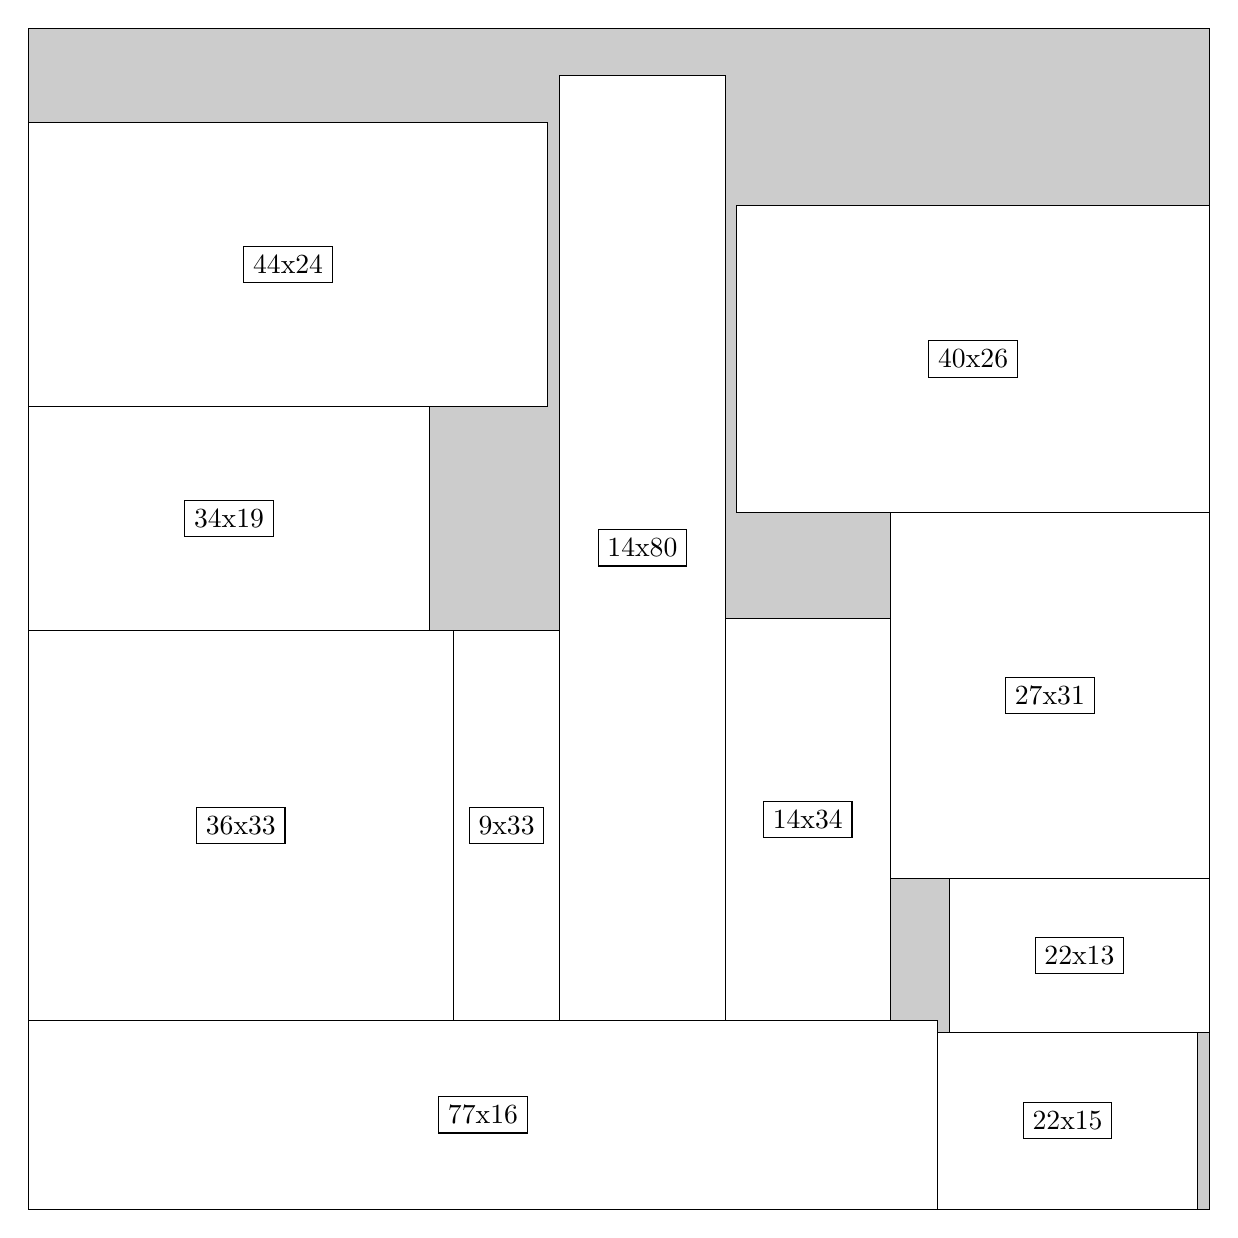
\begin{tikzpicture}[shorten >=1pt,scale=1.0,every node/.style={scale=1.0},->]
\tikzstyle{vertex}=[circle,fill=black!25,minimum size=14pt,inner sep=0pt]
\filldraw[fill=gray!40!white, draw=black] (0,0) rectangle (15.0,15.0);
\foreach \name/\x/\y/\w/\h in {77x16/0.0/0.0/11.549999999999999/2.4,36x33/0.0/2.4/5.3999999999999995/4.95,14x80/6.75/2.4/2.1/12.0,44x24/0.0/10.2/6.6/3.5999999999999996,40x26/9.0/8.85/6.0/3.9,27x31/10.95/4.2/4.05/4.6499999999999995,34x19/0.0/7.35/5.1/2.85,14x34/8.85/2.4/2.1/5.1,22x15/11.549999999999999/0.0/3.3/2.25,9x33/5.3999999999999995/2.4/1.3499999999999999/4.95,22x13/11.7/2.25/3.3/1.95}
\filldraw[fill=white!40!white, draw=black] (\x,\y) rectangle node[draw] (\name) {\name} ++(\w,\h);
\end{tikzpicture}


w =77 , h =16 , x =0 , y =0 , v =1232
\par
w =36 , h =33 , x =0 , y =16 , v =1188
\par
w =14 , h =80 , x =45 , y =16 , v =1120
\par
w =44 , h =24 , x =0 , y =68 , v =1056
\par
w =40 , h =26 , x =60 , y =59 , v =1040
\par
w =27 , h =31 , x =73 , y =28 , v =837
\par
w =34 , h =19 , x =0 , y =49 , v =646
\par
w =14 , h =34 , x =59 , y =16 , v =476
\par
w =22 , h =15 , x =77 , y =0 , v =330
\par
w =9 , h =33 , x =36 , y =16 , v =297
\par
w =22 , h =13 , x =78 , y =15 , v =286
\par
\newpage


\end{document}